\documentclass[sigconf]{acmart}

\usepackage{booktabs} % For formal tables
\usepackage{graphicx}
\usepackage{autobreak}
\usepackage{mytodonotes}
\usepackage{subcaption}
\usepackage[inline]{enumitem}
\usepackage[ruled,vlined]{algorithm2e}
%%%%%%%%%%%%%%%%%%%%%%%%%
\usepackage{cleveref}

% Copyright
%\setcopyright{none}
\setcopyright{acmcopyright}
%\setcopyright{acmlicensed}
%\setcopyright{rightsretained}
%\setcopyright{usgov}
%\setcopyright{usgovmixed}
%\setcopyright{cagov}
%\setcopyright{cagovmixed}


% DOI
\acmDOI{xx.xxx/xxx_x}

% ISBN
\acmISBN{979-8-4007-0629-5/25/03}

%Conference
\acmConference[SAC'25]{ACM SAC Conference}{March 31 –April 4, 2025}{Sicily, Italy}
\acmYear{2025}
\copyrightyear{2025}


\acmArticle{4}
\acmPrice{15.00}

% These commands are optional
%\acmBooktitle{Transactions of the ACM Woodstock conference}
%\editor{Jennifer B. Sartor}
%\editor{Theo D'Hondt}
%\editor{Wolfgang De Meuter}


\begin{document}
\title{Neighbor-Based Decentralized Training Strategies for Multi-Agent Reinforcement Learning}
\titlenote{Produces the permission block, and
  copyright information}
\subtitle{Full Paper}
\subtitlenote{The full version of the author's guide is available as
  \texttt{acmart.pdf} document}
  
\renewcommand{\shorttitle}{SIG Proceedings Paper in LaTeX Format}


%   \institution{University of Bologna}
%   \streetaddress{Via dell'Università, 50}
%   \city{Cesena} 
%   \country{Italy}
% }
% \email{davide.domini@unibo.it}

% \author{Gianluca Aguzzi}
% \affiliation{%
%   \institution{University of Bologna}
%   \streetaddress{Via dell'Università, 50}
%   \city{Cesena} 
%   \country{Italy}\usepackage{algorithm}

% \renewcommand{\shortauthors}{N. Malucelli et al.}

\author{Anonymous Author}
\orcid{1234-5678-9012}
\affiliation{%
  \institution{Anonymous university}
  \country{Anonymous location}
}
% \email{anonymous.author@studio.unibo.it}
\renewcommand{\shortauthors}{A. Author et al.}

\begin{abstract}
Multi-agent deep reinforcement learning (MADRL) is gaining popularity as a powerful extension of
  single-agent reinforcement learning for training collaborative or competitive agents
  in complex environments. 
%
MADRL, however, introduces unique challenges, such as non-stationarity, partial observability, 
  and credit assignment that complicate the learning process.
%
Typically, in the literature, centralized training methods are used to tackle some of these challenges, 
  although they often face scalability limitations as the number of agents grows.
%
For this reason, decentralized training techniques have been proposed, however, 
  generally they have a longer convergence time compared to centralized ones 
  and may lead to instability.
%
This paper investigates the effectiveness of various neighbor-based decentralized training strategies based 
  on the well-known Deep-Q Learning algorithm as a viable alternative to centralized training. 
%  
We evaluate experience sharing, nearest neighboring averaging, and nearest neighboring consensus methods 
  in a custom multi-agent environment and compare their performance against centralized training
  and totally decentralized training. 
%  
Our results show that neighbor-based methods can achieve comparable performance to centralized training 
  while offering improved scalability and communication efficiency. 
%
% Finally, we discuss the trade-offs between these methods and provide insights into their applicability 
%   in different scenarios.
\end{abstract}

%
\begin{CCSXML}
<ccs2012>
 <concept>
  <concept_id>10010520.10010553.10010562</concept_id>
  <concept_desc>Computer systems organization~Embedded systems</concept_desc>
  <concept_significance>500</concept_significance>
 </concept>
 <concept>
  <concept_id>10010520.10010575.10010755</concept_id>
  <concept_desc>Computer systems organization~Redundancy</concept_desc>
  <concept_significance>300</concept_sigagentnificance>
 </concept>
 <concept>
  <concept_id>10010520.10010553.10010554</concept_id>
  <concept_desc>Computer systems organization~Robotics</concept_desc>
  <concept_significance>100</concept_significance>
 </concept>
 <concept>
  <concept_id>10003033.10003083.10003095</concept_id>
  <concept_desc>Networks~Network reliability</concept_desc>
  <concept_significance>100</concept_significance>
 </concept>
</ccs2012>  
\end{CCSXML}

\ccsdesc[500]{Computer systems organization~Embedded systems}
\ccsdesc[300]{Computer systems organization~Redundancy}
\ccsdesc{Computer systems organization~Robotics}
\ccsdesc[100]{Networks~Network reliability}


\keywords{Multi-Agent Reinforcement Learning, Decentralized Training, Neighbor-Based Methods, Scalability, Communication Efficiency}
\maketitle

\section{Introduction}
The increasing complexity of real-world systems, from robotic swarms to smart grids, demands intelligent control strategies capable of adapting to dynamic and often unpredictable environments.
%
In this direction, \emph{reinforcement learning} (RL)~\cite{sutton2018reinforcement} has emerged as a powerful paradigm for training agents to interact with their environment and learn optimal policies through trial and error.
%
Moving beyond single-agent settings, \emph{multi-agent reinforcement learning} (MARL)~\cite{bucsoniu2010multi} extends RL to scenarios where multiple agents must collaborate or compete to achieve a common goal.
%
Recent advances in deep learning have further revolutionized the field, 
enabling the training of complex policies in high-dimensional state and action spaces, 
leading to the emergence of \emph{multi-agent deep reinforcement learning} (MADRL)~\cite{gronauer2022multi}.
%
MADRL has gained significant traction due to its flexibility and capacity to learn diverse behaviors, 
ranging from cooperative~\cite{gupta2017cooperative} to competitive~\cite{tampuu2017multiagent}, 
as demonstrated in various case studies involving video games~\cite{shao2019survey}, robotics~\cite{orr2023multi},
and traffic management. 
%
This paper focuses on the subdomain of \emph{cooperative multi-agent reinforcement learning}, 
a particularly active and impactful area of research within MADRL~\cite{oroojlooy2023review}.

\sloppy
Many prominent approaches in this field employ a centralized training and decentralized execution paradigm
 (e.g.,MAPPO~\cite{yu2022surprising}, MADDPG~\cite{DBLP:conf/nips/LoweWTHAM17}, QMIX~\cite{DBLP:conf/icml/RashidSWFFW18}, QTRAN~\cite{DBLP:conf/icml/SonKKHY19}), 
 where a centralized learner trains distributed policies that are subsequently executed independently. 
 While facilitating decentralized runtime operation and avoiding single points of failure, 
 this approach typically entails an offline learning phase (using simulators and centralized computation) 
 followed by online execution with no further learning. 
 This inherent limitation hinders adaptation to changing environments or tasks at runtime.  
% 
While fully independent learners~\cite{abed2016comparison} offer a potential solution for online learning,
 they often underperform centralized counterparts due to instability in training and a lack of differentiation between agents and their interactions with the environment. 
%
However, in many real-world multi-agent systems, 
 agents only interact with a limited subset of the overall system (also called \emph{networked agents}),
 as exemplified by limited sensing ranges in swarm robotics or localized interactions.  
 This observation also holds true in other natural systems, such as animal herds.
%
Therefore, 
this paper proposes and formalizes a family of distributed learning methodologies based on neighborhood information.
This approach aims to: 
i) incorporate richer information compared to independent learners, and
ii) facilitate the emergence of collective behaviors through local interactions between networked agents.
Specifically, we investigate three distinct neighboring-based training strategies encompassing both neural network-based approaches 
(e.g., neighboring averaging and consensus) 
and experience-based methods inspired by centralized experience sharing~\cite{DBLP:conf/nips/ChristianosSA20}. 
We demonstrate the effectiveness of these strategies in comparison to both centralized and fully distributed approaches, 
highlighting how neighborhood-based policies offer a compelling compromise between these two extremes.

The remainder of this paper is structured as follows.
Section~\ref{sec:background} provides an overview of multi-agent reinforcement learning,
highlighting the key challenges and training paradigms.
Section~\ref{sec:neighboring} introduces the proposed neighboring-based training strategies,
detailing their implementation and operation.
Section~\ref{sec:experiments} presents the experimental setup and evaluation metrics.
Section~\ref{sec:results} discusses the results of the experiments,
comparing the performance of the neighboring-based methods against centralized training.
Finally, Section~\ref{sec:conclusion} concludes the paper,
summarizing the key findings and outlining potential future research directions.

\section{Background and Motivation}\label{sec:background}
MARL is an extension of a sequential decision-making process, 
where multiple \emph{agents} interact with each other and a shared \emph{environment}.
In particular, each agent in the system aims to maximize its own \emph{reward signal} (i.e., a scalar feedback signal),
which is typically a function of the global state (sometime not known, making the system \emph{partial observable}) and the joint action taken by all agents.
%
In doing that, each agent perceive the environment through its own \emph{observation function},
which maps the global state to the agent's local observation and perform an action based on its \emph{policy} (i.e., a mapping from observations to actions).
%
This chosen action is then combined with the actions of other agents forming a \emph{joint action},
which is used to update the global state and reward.
 
In this paper, we focus on cooperative MADRL scenarios (so the deep version of MARL), 
where agents must collaborate to achieve a common goal.
In the following, we provide an overview of the key concepts in MADRL, 
including the formalization of the problem, the deep Q-learning algorithm, and the training paradigms used in the literature.
\subsection{Formalization}
Since MADRL is a broad field, it is essential to provide a formalization to guide the discussion.
In this paper, we consider partially observable networked markov decision process (PONMDP)~\cite{DBLP:journals/tac/AdlakhaLG12} as a tuple $(\mathcal{G}, \mathcal{S}, \mathcal{A}, \mathcal{O}, \mathcal{P}, \mathcal{R}, \gamma)$, where

\begin{itemize}
  \item $\mathcal{G} = (N, E)$ is a communication graph, where $N$ is the set of $n$ agents and $E \subseteq N \times N$ represents the communication links between agents. Time-varying graphs $\mathcal{G}_t = (N, E_t)$ can be used to represent communication evolving over time $t$.
  \item $\mathcal{S}$ is the global state space.
  \item $\mathcal{A} = \mathcal{A}^1 \times \dots \times \mathcal{A}^n$ is the joint action space, where $\mathcal{A}^i$ is the action space of agent $i$.
  \item $\mathcal{O} = \mathcal{O}^1 \times \dots \times \mathcal{O}^n$ is the joint observation space, where $\mathcal{O}^i$ is the observation space for agent $i$.
  \item $\mathcal{P}: \mathcal{S} \times \mathcal{A} \times \mathcal{S} \to [0, 1]$ is the state transition function, describing the probability of transitioning to a new state $s' \in \mathcal{S}$ given the current state $s \in \mathcal{S}$ and joint action $a \in \mathcal{A}$.
  \item $\mathcal{R} = {\mathcal{R}^i}_{i \in N}$, where $\mathcal{R}^i: \mathcal{S} \times \mathcal{A} \to \mathbb{R}$ is the reward function for agent $i$.
  \item $\gamma \in [0, 1]$ is the discount factor.
\end{itemize}
Each agent $i$ at time $t$ receives an observation $o^i_t \in \mathcal{O}^i$, 
takes an action $a^i_t \in \mathcal{A}^i$ based on its local policy $\pi^i: \mathcal{O}^i \times \mathcal{A}^i \to [0,1]$, and receives a reward $r^i_{t+1} = \mathcal{R}^i(s_t, a_t)$. 
%
The global state evolves according to $\mathcal{P}$. 
Agents can exchange information with their neighbors in $\mathcal{G}$ 
(or $\mathcal{G}t$ if the graph is time-varying). 
%
The objective is typically to maximize the expected discounted sum of rewards $\sum{t=0}^{\infty} \gamma^t r^i_t$ for each agent $i$, 
or some global reward function like the average reward over all agents.
Formally, it can be defined as:
\[ J(\{\pi^i\}) = \lim_{T \to \infty} \mathbb{E} \left[ \frac{1}{T} \sum_{t=0}^{T-1} \frac{1}{N} \sum_{i \in \mathcal{N}} R^i(s_t, a_t) \right] \]

In doing this, agents typically use other function to estimate the value of taking an action in a given state, such as the action-value function or Q-value. 
The latter represents the expected cumulative discounted reward the agent will receive by taking action $a \in \mathcal{A}$ in state $s \in \mathcal{S}$ and then following its policy $\pi^i$:

\[ Q^i(s, a) = \mathbb{E}_{\pi^i} \left[ \sum_{t=0}^{\infty} \gamma^t r^i_{t+1} | s_0 = s, a_0 = a \right] \]

%Similar to the individual reward function, a global average reward function can be defined as $\bar{\mathcal{R}}(s, a) = \frac{1}{n} \sum_{i=1}^n \mathcal{R}^i(s,a)$, leading to a global average Q-value:

%\[ \bar{Q}(s, a) = \mathbb{E}_{\pi} \left[ \sum_{t=0}^{\infty} \gamma^t \bar{\mathcal{R}}(s_t, a_t) | s_0 = s, a_0 = a \right] \]

%where $\pi = \{\pi^i\}_{i \in N}$ represents the joint policy. 
%The goal in collaborative MARL is often to find a joint policy that maximizes this global average Q-value or a similar global objective.
There are several algorithms which try to find the optimal Q-value function, one of the most popular is the deep Q-learning algorithm.
\subsubsection{Deep Q-Learning Formalization}
Deep Q-learning~\cite{DBLP:conf/l4dc/FanWXY20} utilizes a deep neural network, 
often referred to as a Q-network, to approximate the action-value function $Q(s, a)$. 
This network takes the state $s$ as input and outputs a vector of Q-values, one for each possible action $a \in \mathcal{A}$.  
The optimal action-value function, denoted $Q^*(s, a)$, satisfies the Bellman optimality equation:

\[ Q^*(s, a) = \mathbb{E}_{s' \sim \mathcal{P}} \left[ r + \gamma \max_{a'} Q^*(s', a') | s, a \right] \]

where $\mathcal{P}$ is the state transition probability distribution.  
Deep Q-learning aims to train the Q-network to approximate $Q^*(s, a)$ by minimizing the loss function:

\[ \mathcal{L}(\theta) = \mathbb{E}_{(s, a, r, s') \sim \mathcal{D}} \left[ \left( r + \gamma \max_{a'} Q(s', a'; \theta^-) - Q(s, a; \theta) \right)^2 \right] \]

where $\theta$ are the parameters of the Q-network, $\theta^-$ are the parameters of a target Q-network (used for stability), 
and $\mathcal{D}$ is the experience replay buffer, a collection of past experiences $(s, a, r, s')$.
%
In the multi-agent setting, each agent $i$ has its own Q-network $Q^i(o^i, a^i; \theta^i)$ that takes its local observation $o^i$ as input.  
For centralized training, the global state $s$ can be used as input. 
The specific form of the multi-agent Q-function and the update rules depend on the chosen MARL algorithm (e.g., distributed deep Q-learning~\cite{ong2015distributed}, value decomposition methods~\cite{DBLP:conf/icml/SonKKHY19}).  
For example, in independent deep Q-learning, each agent updates its Q-network independently using its local reward $r^i$:
\begin{equation}
  \resizebox{\linewidth}{!}{$
  \mathcal{L}^i(\theta^i) = \mathbb{E}_{(o^i, a^i, r^i, o'^i) \sim \mathcal{D}^i} \left[ \left( r^i + \gamma \max_{a'^i} Q^i(o'^i, a'^i; \theta^{i-}) - Q^i(o^i, a^i; \theta^i) \right)^2 \right]
  $}
  \end{equation}
%\subsection{Key Concepts}

\subsection{Learning Schemes}
\begin{figure}
  \centering
  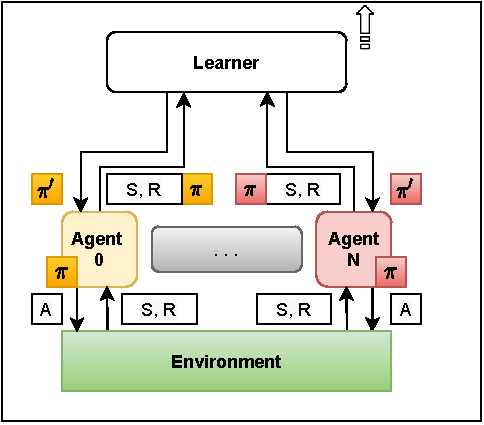
\includegraphics[width=0.49\linewidth]{figures/learning-scheme-ctde.pdf}
  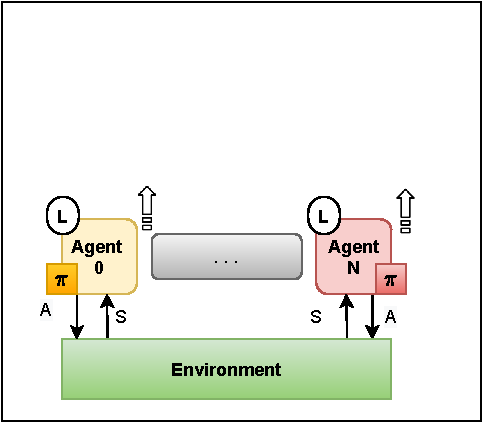
\includegraphics[width=0.49\linewidth]{figures/learning-scheme-dtde.pdf}
  \caption{Graphical representation of centralized training with decentralized execution (left) and decentralized training with decentralized execution (rigth) in multi-agent reinforcement learning.}
  \label{fig:learning_paradigms}
\end{figure}
Multi-agent learning can be categorized based on the training scheme and the information accessibility for agents. 
Two prominent paradigms are centralized training with decentralized execution (CTDE) and decentralized training with decentralized execution (DTDE)---see \Cref{fig:learning_paradigms}.

\paragraph{Centralized Training with Decentralized Execution (CTDE)}
In CTDE, a central learner trains all agents, 
but execution of the learned policy is decentralized. 
This process typically involves two phases:
\begin{itemize}
    \item \textbf{Offline training:} agents interact with a simulator or environment, 
    gathering experience data used to update the central learner's policy.
    \item \textbf{Online execution:} agents deploy the learned policy in the environment without further learning.
\end{itemize}
This approach offers several benefits.  
Leveraging a centralized dataset allows for efficient learning, 
potentially exploiting global information, 
which is crucial in cooperative scenarios requiring coordinated actions. 
Furthermore, decentralized execution allows agents to act independently after training.
%
However, CTDE has limitations. 
Scalability can become problematic with a large number of agents. 
The reliance on a central learner hinders adaptation to dynamic environments or tasks during runtime.
\sloppy
\paragraph{Decentralized Training with Decentralized Execution (DTDE)}
DTDE eliminates the central learner; each agent learns independently. 
Inter-agent cooperation and communication can be incorporated during both training and execution. 
Unlike CTDE, training and execution phases are not necessarily separate. 
Simultaneous learning and execution allow for adaptation to changing environments or tasks at runtime.
%
Key advantages of DTDE include scalability with the number of agents and adaptability to dynamic environments.
%
However, DTDE faces challenges. 
Convergence time is often longer compared to centralized training. 
The lack of central coordination can lead to instability and difficulties in differentiating agents and their environmental interactions. 
Online learning in DTDE can introduce non-stationarity if agents do not account for other agents' evolving policies during training, 
as the environment effectively changes from each agent's perspective.

\subsection{State of the Art}
Multi-agent reinforcement learning is a longstanding research area with a rich literature, starting 
from seminal works like~\cite{tan1993multi} and~\cite{busoniu2008comprehensive} to more recent contributions like~\cite{gronauer2022multi} and~\cite{canese2021multi}.
%
In the following, we briefly discuss some of the most relevant approaches in the field.
\subsubsection{Independent Learners}
In independent learners, each agent learns its policy independently, disregarding the actions and policies of other agents. 
This straightforward approach, among the earliest explored in MARL, often relies on variants of Q-learning. 
However, independent learners struggle with coordination due to the non-stationarity introduced by the simultaneous learning of other agents.

Several algorithms have attempted to address these coordination challenges within the independent learner paradigm. 
Basic decentralized Q-learning~\cite{tan1993multi} allows each agent to learn its Q-values independently but often converges to suboptimal joint policies due to a lack of coordination. 
Subsequent work introduced heuristic-based extensions to improve coordination.
Approaches like distributed Q-learning~\cite{lauer2000algorithm} incorporate optimism in Q-value updates and equilibrium selection mechanisms to mitigate the convergence to shadowed equilibria (i.e., equilibria that are unstable due to the independent learning processes). 
Instead, algorithms such as hysteretic Q-learning~\cite{matignon2007hysteretic}, lenient Q-Learning~\cite{bloembergen2010lenient} and win-or-learn fast policy hill climbing~\cite{bowling2002multiagent} employ adaptive learning rates to address the issue of alternating exploration between agents, improving robustness and convergence.
%
Empirical comparisons of these algorithms highlight the trade-offs in performance across various MARL tasks and coordination challenges~\cite{matignon2012independent}. 
While initially developed for tabular settings, some of these methods, like hysteretic Q-learning~\cite{palmer2017lenient} and lenient Q-learning, have been extended to deep reinforcement learning settings. 
However, these independent approaches, even with deep learning, often exhibit instability and slow convergence in complex environments and fundamentally lack explicit mechanisms for inter-agent coordination. 
Consequently, more sophisticated MARL algorithms have been developed that explicitly account for the interactions and policies of other agents to facilitate more effective coordination.
\paragraph{Neighboring-Based Methods}
Neighboring-based methods in MARL address the scalability and communication overhead challenges of fully centralized approaches by restricting agent interactions to a local neighborhood. 
This introduces a structure where agents communicate and coordinate with a limited set of neighbors, reducing the complexity of joint action and policy learning.
%
One prominent category within neighboring-based methods is consensus-based algorithms. 
These algorithms aim to reach a consensus among agents on shared values or policies through local information exchange. 
Early work like QD-learning~\cite{kar2012qd} extends Q-learning with a consensus update term, 
enabling agents to converge towards optimal Q-values despite only receiving local rewards.
%  
Recent advances in consensus-based MARL leverage deep learning and actor-critic architectures, 
combining local policy updates with consensus updates on critic parameters or gradients, 
as seen in the recent works~\cite{7434032,pennesi2010distributed,zhang2018fully,DBLP:journals/jmlr/CiosekW20}.

These algorithms often exhibit improved scalability and communication efficiency compared to fully centralized methods, 
but still need lack in capturing the global structure of the environment and the interactions between agents.

\paragraph{Centralized Training Methods} CTDE is a prominent paradigm in MARL~\cite{ning2024survey}, 
leveraging centralized information during training to learn decentralized policies for execution. 
This approach addresses the challenges of partial observability and non-stationarity while maintaining the scalability of decentralized execution. % 
Actor-critic methods are well-suited for the CTDE paradigm, 
where a centralized critic provides feedback to decentralized actors~\cite{DBLP:conf/icml/RashidSWFFW18,DBLP:journals/corr/SunehagLGCZJLSL17,yu2022surprising,DBLP:conf/nips/LoweWTHAM17}. 
% 
The most influential algorithms in this area are the one called policy-based methods (i.e., the ones that learn a policy directly).
%
Multi-agent deep deterministic policy Gradient (MADDPG)~\cite{DBLP:conf/nips/LoweWTHAM17} employs a centralized critic that has access to the states and actions of all agents, providing more informative feedback for policy updates. 
Each agent then learns a deterministic policy based on its local observations. % 
Building on the actor-critic framework, Multi-Agent Proximal Policy Optimization (MAPPO)~\cite{yu2022surprising} extends the centralized critic concept to the policy optimization setting. 
MAPPO leverages a centralized critic to estimate advantage functions for policy updates, while individual agents learn stochastic policies. 
This approach has shown promising results in various cooperative and competitive MARL tasks, exhibiting improved sample efficiency and robustness compared to MADDPG. % 
Another class of algorithms, called value-based methods, learn a value function that estimates the expected return for each agent.
%
Value Decomposition Networks (VDN)~\cite{DBLP:journals/corr/SunehagLGCZJLSL17} and QMIX~\cite{DBLP:conf/icml/RashidSWFFW18} are representative algorithms in this category. 
VDN factorizes the joint Q-function into a sum of individual agent Q-functions, simplifying the learning process. 
QMIX improves upon VDN by learning a monotonic mixing function that combines individual Q-values, 
allowing for more complex representations of joint action values. % 

Another approach to address the scalability challenge in MARL is \emph{mean field reinforcement learning}, i.e., the one that models the interaction between agents through a mean field, simplifying the multi-agent problem into a single-agent problem against an average opponent.
%
In this context, mean field q-learning (Mean-Q)~\cite{DBLP:conf/icml/YangLLZZW18} has been proposed.
This approach scales well to large numbers of agents and has been successful in various applications. 
% 
There are also modern solution which leverages collective abstraction to reduce the complexity of the problem, such as the one proposed in field-informed reinforcement learning~\cite{DBLP:conf/acsos/AguzziVE23}.
\subsection{Motivation}
MADRL faces a critical challenge in balancing scalability and performance.  
Centralized training methods, while effective, often suffer from computational bottlenecks and difficulties scaling to large numbers of agents. 
While distributed training approaches offer improved scalability, 
they frequently assume independent learners, 
neglecting crucial inter-agent coordination and leading to suboptimal global performance.  
%
Neighbor-based methods have shown promise in simpler, tabular settings by enabling localized coordination,
but their integration with deep reinforcement learning remains largely unexplored. 
This work bridges this gap by introducing a novel approach that combines the power of deep learning with the scalability of neighbor-based communication.  
Our method aims to achieve both efficient decentralized learning and effective coordination, enabling online adaptation and robust performance in complex multi-agent environments.
\section{Neighboring-Based Distributed Learning Strategies}\label{sec:neighboring}
This section introduces three neighboring-based distributed learning strategies for multi-agent reinforcement learning. 
These strategies leverage local interactions between agents to improve learning efficiency and coordination.
For this investigation, we focus on deep Q-learning as the underlying learning algorithm,
and we consider the following strategies:
 k-nearest neighbor averaging, k-nearest neighbor consensus, and experience sharing.


Since these strategies are in general based on the notion of k-nearest neighbors,
we first introduce this concept and then describe each strategy in detail.
Formally, consider a \emph{weighted} communication graph $\mathcal{G} = (N, E, W)$, where $N$ is the set of agents, where $W: E \rightarrow \mathbb{R}^+$ is a weight function assigning a positive weight to each edge.  
Let $d(i,j)$ denote the shortest path length between agents $i$ and $j$ in the weighted graph $\mathcal{G}$. 
This can be calculated, for instance, using Dijkstra's algorithm. 
The length of a path is the sum of the weights of the edges along the path. If no path exists between $i$ and $j$, we set $d(i,j) = \infty$.
%
Then, the set of $k$-nearest neighbors of agent $i$ is defined as:
$$ \mathcal{N}_k(i) = { j \in N \setminus {i} \mid \text{rank}(d(i,j)) \leq k } $$
where $\text{rank}(d(i,j))$ denotes the rank of the distance $d(i,j)$ among all distances from agent $i$ to other agents in $N \setminus {i}$, sorted in ascending order (e..g, $\text{rank}(d(i,j)) = 1$ for the smallest distance).
Ties can be broken arbitrarily.

\subsection{K-Nearest Neighbor Averaging}
This approach averages an agent's Q-values with those of its nearest neighbors. 
Each agent maintains a local Q-network and shares its Q-values with its neighbors. 
The neighbors average the received Q-values and use the result to update their own Q-networks. 
This leverages the collective knowledge of neighboring agents to improve learning.
%
Formally, giving $\theta^t_i, i \in N$ the parameters of the Q-networks of the agent $i$ at the time $t$,
the update rule for agent $i$ at time $t+1$ is:
\begin{equation}
  \theta^{t+1}_i = \theta^t_i + \alpha \sum_{j \in \mathcal{N}_k(i)} \frac{1}{k} \theta^t_j
\end{equation}

\subsection{K-Nearest Neighboring Consensus}
In case of homogeneous agents (i.e., when all agents have the same action and observation space),
the goal of learning is to find a common policy that all agents can follow.
This approach is typically used in large-scale systems where agents are identical and need to reach a consensus---see [cite].
%
In this case, instead of forcing a common policy, we can let agents learn independently and then select the best-performing agent as the reference for the others, leading to a consensus on the best policy.
%
In this way, each agent $i$ continue to learn independently, but at each iteration, it updates its Q-network using the Q-values of the best-performing agent in its neighborhood.

The best performing agent is selected based on the average reward it has received in the last $n$ episodes.
Formally, the update rule for agent $i$ at time $t+1$ is:
\begin{equation}
  \theta^{t+1}_i \leftarrow \theta^t_{\text{best}}
\end{equation}
where $\theta^t_{\text{best}}$ is the Q-network of the best-performing agent in the neighborhood $\mathcal{N}_k(i)$ at time $t$.

\subsection{Experience Sharing}
Experience sharing is a simple yet effective method for distributed learning.
This approach is typically used in centralized training to improve sample efficiency and learning stability.
In our distributed setting, each agent maintains its own experience replay buffer, but it also shares a fraction of its experiences with its neighbors.
This allows agents to learn from each other's experiences, potentially accelerating learning and improving coordination because agents can learn from each other's mistakes and successes.
%
Formally, the reply buffer of agent $i$ at time $t$ is $\mathcal{D}^t_i = \{(o^i, a^i, r^i, o'^i)\}$.
At each iteration, agent $i$ shares a fraction $\beta$ of its experiences with its neighbors in $\mathcal{N}_k(i)$.
The update rule for agent $i$ at time $t+1$ is:
\begin{equation}
  \mathcal{D}^{t+1}_i = \mathcal{D}^t_i \cup \bigcup_{j \in \mathcal{N}_k(i)} \beta \mathcal{D}^t_j
\end{equation}
\subsection{Neighboring-Based Training with Deep Q-Learning}
The neighboring-based training strategies can be integrated with deep Q-learning to enable distributed learning in multi-agent settings.
%
The algorithm follow the same structure as the deep Q-learning algorithm, but with the addition of the neighboring-based intereactions.
%
This may happen with a different frequency for each strategy, depending on the communication overhead and the desired level of coordination.

In \Cref{alg:neighbor_dqn} we provide a detailed description of the integration of the neighboring-based strategies with deep Q-learning.
\begin{algorithm}
  \caption{Neighboring-Based Deep Q-Learning}
  \label{alg:neighbor_dqn}
  \ForEach{agent $i \in N$}{
      Initialize Q-network $Q^i(o^i, a^i; \theta^i)$ and target network $Q^{i-}(o^i, a^i; \theta^{i-})$\\
      Initialize replay buffer $\mathcal{D}^i$
  }
  \For{episode = 1 to M}{
      \ForEach{agent $i \in N$}{
          Initialize initial observation $o_0^i$
      }
      \For{t = 0 to T}{
          \ForEach{agent $i \in N$}{
              Select action $a_t^i$ based on $\epsilon$-greedy policy using $Q^i(o_t^i, a^i; \theta^i)$\\
              Execute action $a_t^i$ and observe reward $r_{t+1}^i$ and next observation $o_{t+1}^i$\\
              Store $(o_t^i, a_t^i, r_{t+1}^i, o_{t+1}^i)$ in $\mathcal{D}^i$\\
              Sample a mini-batch from $\mathcal{D}^i$\\
              Calculate target values using chosen neighboring strategy (see below)\\
              Update $\theta^i$ by minimizing the TD error\\
              Every C steps, update target network $\theta^{i-} \leftarrow \theta^i$\\
              \textbf{
              Every S steps, perform neighbor interaction (e.g., averaging, consensus, experience sharing)}
          }
      }
  }
\end{algorithm}
\section{Experimental Setup}\label{sec:experiments}

To validate our approach, we developed a custom learning scenario using three State-of-the-Art frameworks 
  in Reinforcement Learning and Deep Learning, namely: \emph{Ray}~\cite{DBLP:conf/osdi/MoritzNWTLLEYPJ18} 
  (in particular, its module \emph{RLlib}~\cite{DBLP:conf/icml/LiangLNMFGGJS18}),
  \emph{Gymnasium}~\cite{DBLP:journals/corr/abs-2407-17032}
  and \emph{PyTorch}~\cite{DBLP:conf/nips/PaszkeGMLBCKLGA19}.

First, we extended the \texttt{MultiAgentEnv} from RLlib to implement a custom cooperative environment 
  called \emph{collect the items} -- see \Cref{fig:env}.
%
This environment consists of a 2D euclidean space in which a variable number of \emph{items} and \emph{agents} 
 are randomly placed.
%
The goal of the agents is to cooperate to collect all the items in the smallest amount of time possible. 
%
In particular, each agent has an observation space defined by three main parameters, namely: 
\begin{enumerate*}[label=(\roman*)]
  \item number of closest agents that the agent is able to see (thus, forming a neighborhood);
  \item number of closest items that the agent is able to see;
  \item memory of past states, thus encoding also temporal information, helping each agent to understand 
    the evolution of the environment.
\end{enumerate*} 
%
Regarding the action space, each agent has $8$ possible moves, namely the possible direction on a grid 
  (up, down and diagonal).

% Reward 



% Specify the chosen RL algorithm (DQN) and its hyperparameter configuration

% Define the evaluation metrics: average episode length and average reward

\begin{figure}
  \centering
  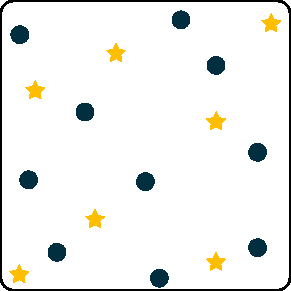
\includegraphics[width=0.7\linewidth]{figures/env.pdf}
  \caption{Graphical representation of the environment. 
  Specifically, the environment consists of a 2D euclidean space.
  The blue dots represent the agents, while the yellow stars represent the items that 
  the agents aim to collect.
  }
  \label{fig:env}
\end{figure}

\begin{figure}
  \centering
  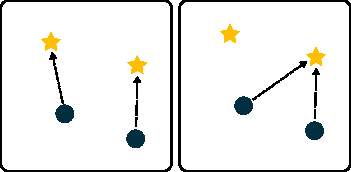
\includegraphics[width=1\linewidth]{figures/behavior.pdf}
  \caption{Graphical representation of wanted and unwanted behaviors.
  On the left, the wanted behavior, the agents correctly cooperate to cover
  two different items.
  While, on the right, the agents do not correctly cooperate covering
  the same item.
  }
  \label{fig:behavior}
\end{figure}


\section{Results and Evaluation}\label{sec:results}
\begin{itemize}
\item \textbf{Performance comparison:}
\begin{itemize}
\item Present the results of each distributed strategy against the centralized training baseline.
\item Use graphs and statistical analysis to compare the average episode length and average reward.
\item Highlight which neighbor-based methods perform comparably to centralized training.
\end{itemize}
\item \textbf{Scalability analysis:}
\begin{itemize}
\item Describe how the experiments were modified to assess scalability (increasing agents, spawn area).
\item Show how each method scales with the increasing complexity, using appropriate visualizations.
\item Discuss the implications of using pre-trained models with a larger number of agents.
\end{itemize}
\item \textbf{Communication overhead analysis:}
\begin{itemize}
\item Quantify the amount of information exchange for each strategy.
\item Compare the communication overhead across different neighborhood sizes, possibly using graphs.
\item Discuss the trade-offs between performance and communication efficiency.
\item Mention potential techniques for reducing communication overhead.
\end{itemize}
\end{itemize}

\begin{figure}
  \centering
  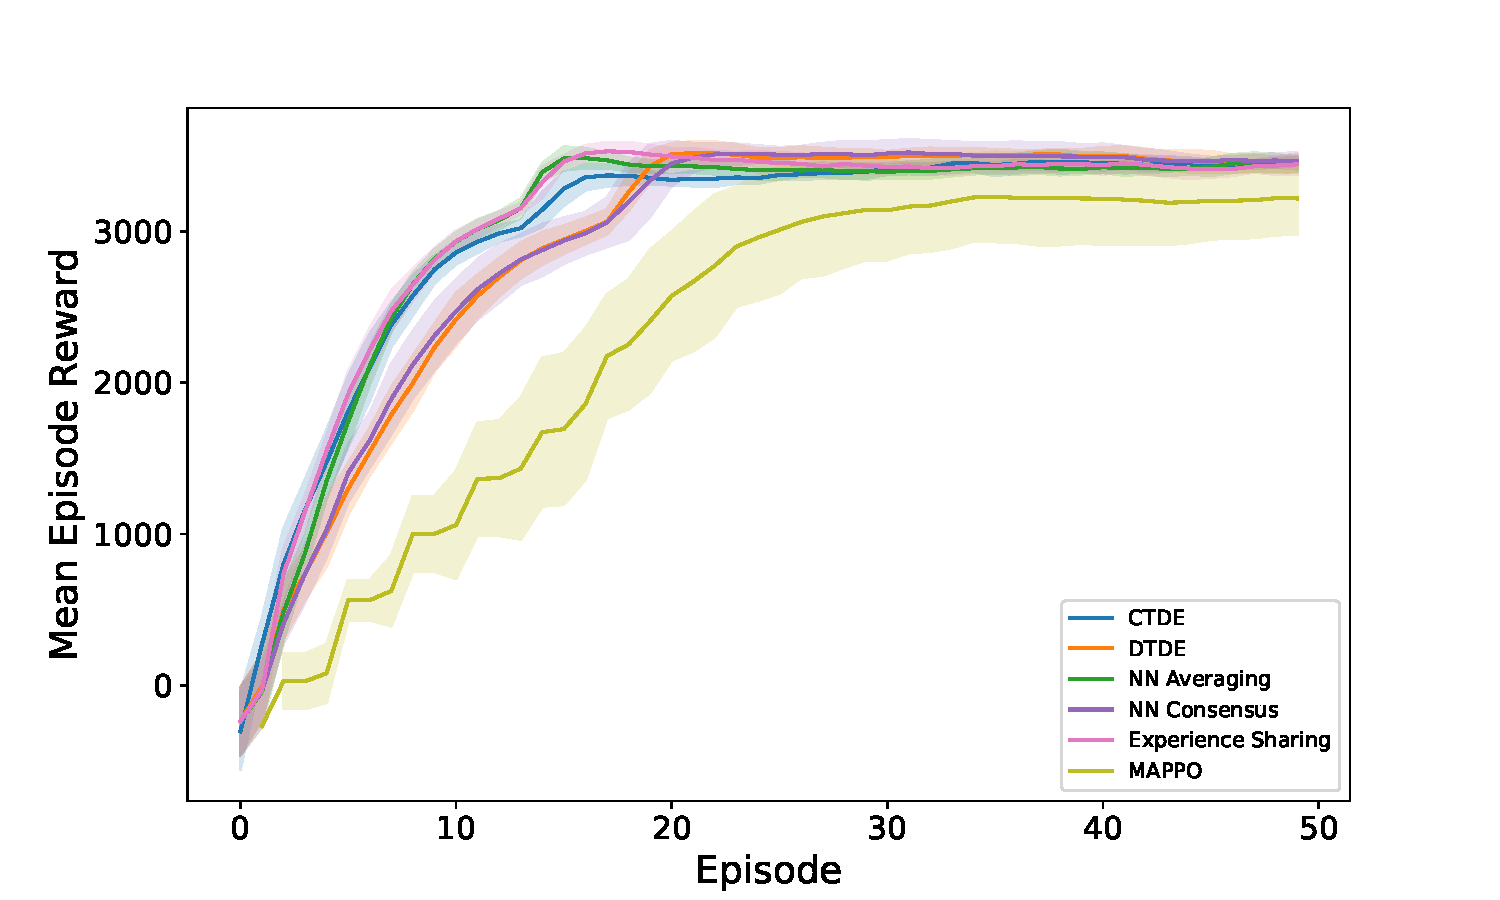
\includegraphics[width=1\linewidth]{figures/episode_reward_mean.pdf}
  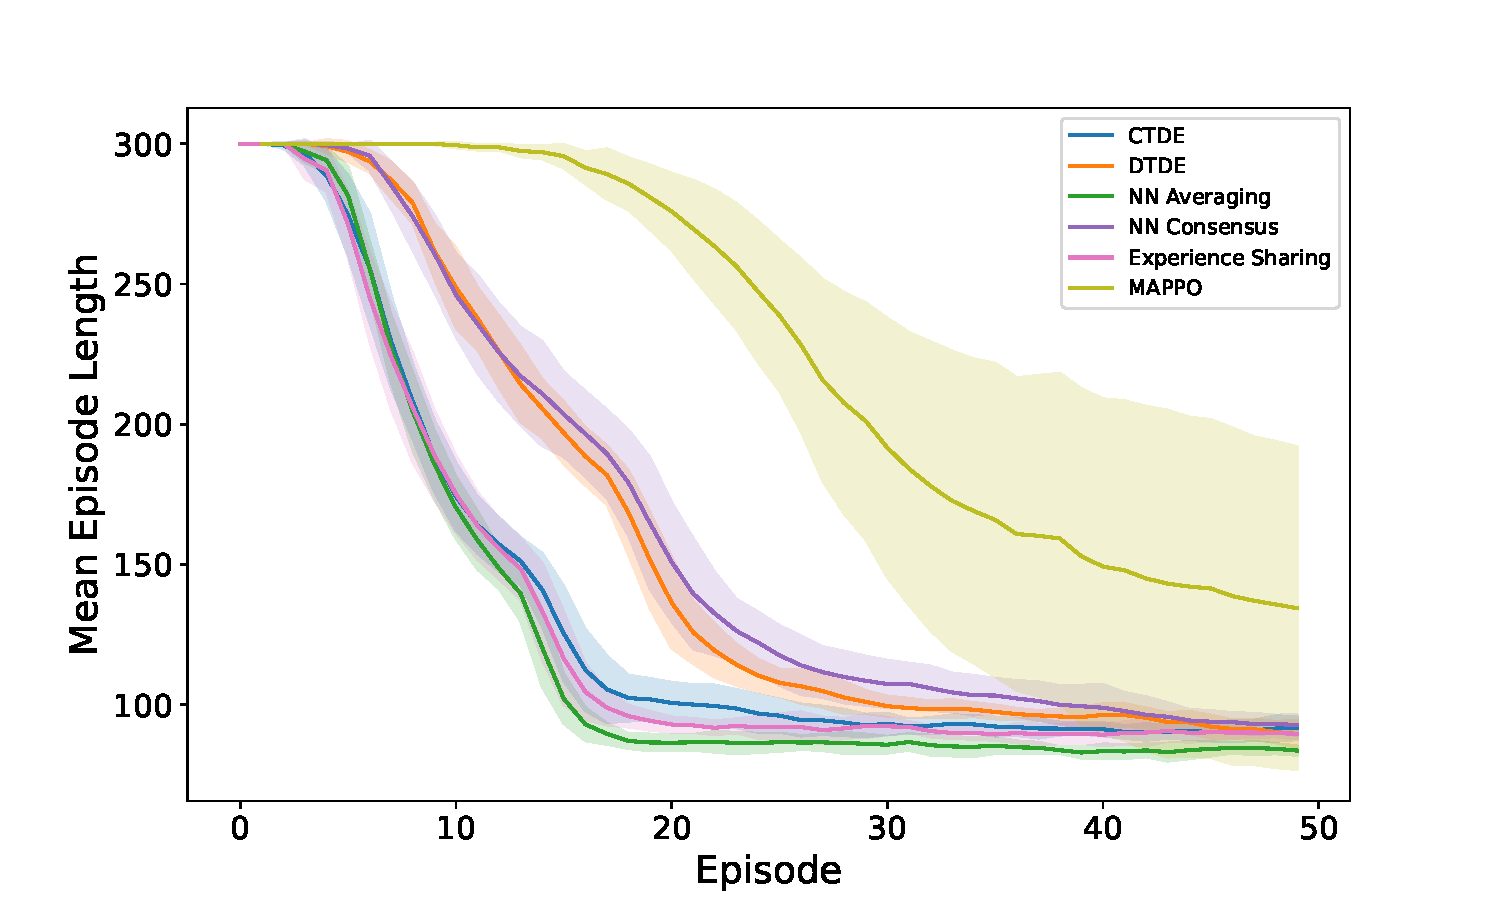
\includegraphics[width=1\linewidth]{figures/episode_len_mean.pdf}
  \caption{Training results...}
  \label{fig:results}
\end{figure}

\begin{figure*}[htb]
  \centering
  \begin{subfigure}[b]{0.3\textwidth}
      \centering
      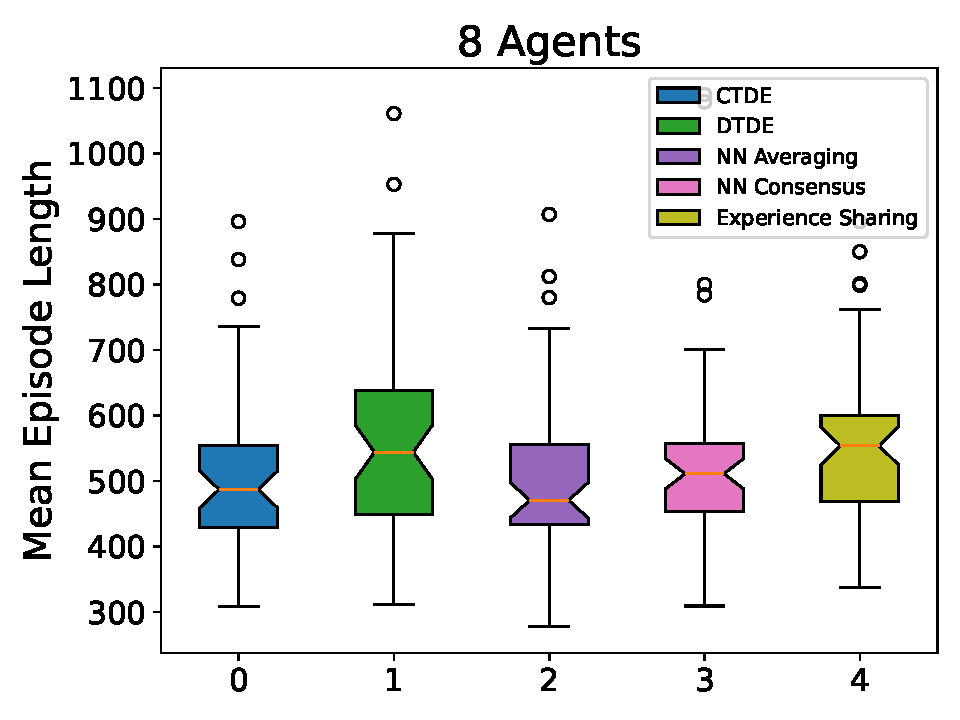
\includegraphics[width=\textwidth]{figures/mean-time-comparison-8-agents.pdf}
      %\caption{Start of the simulation.}
      % \label{fig:zones1}
  \end{subfigure}
  \begin{subfigure}[b]{0.3\textwidth}
      \centering
      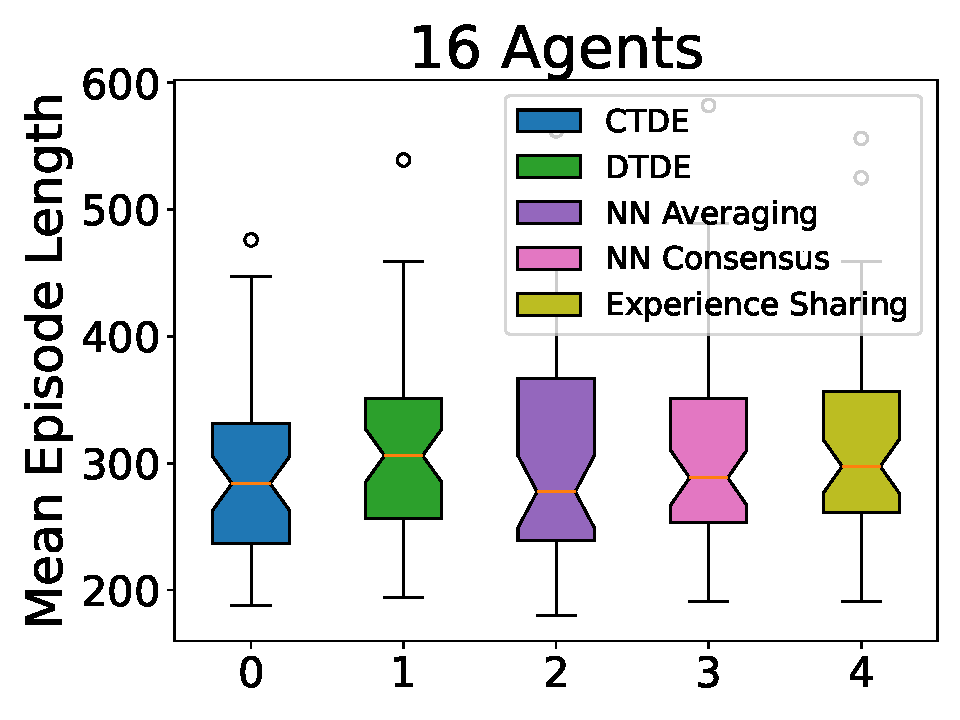
\includegraphics[width=\textwidth]{figures/mean-time-comparison-16-agents.pdf}
      %\caption{After k time steps of the simulation.}
      % \label{fig:zones2}
  \end{subfigure}
  \begin{subfigure}[b]{0.3\textwidth}
      \centering
      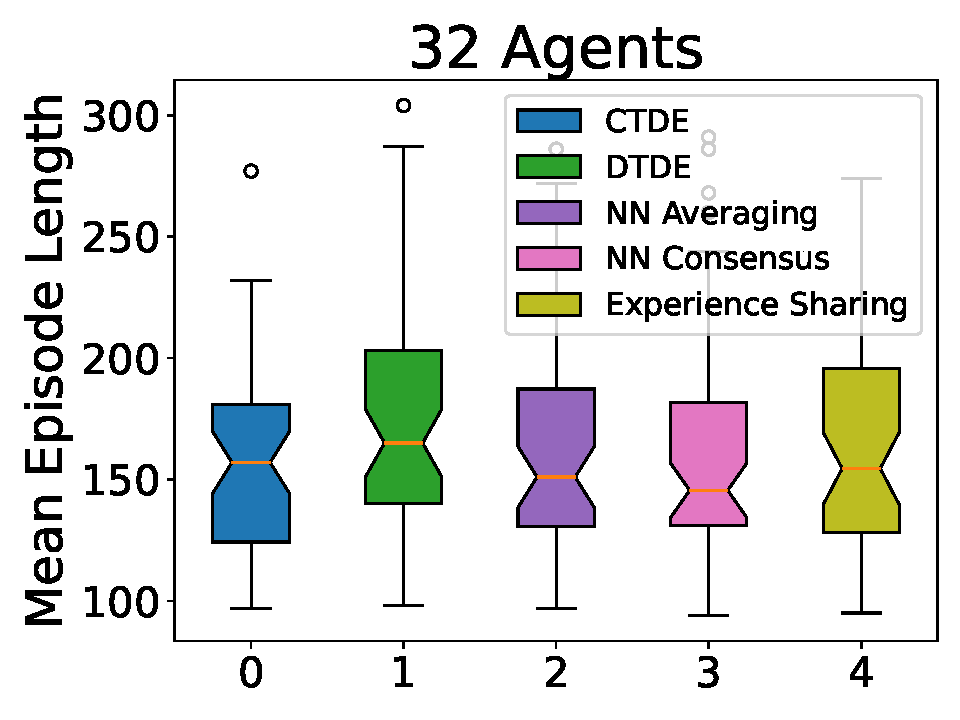
\includegraphics[width=\textwidth]{figures/mean-time-comparison-32-agents.pdf}
      %\caption{End of the simulation.}
      % \label{fig:zones3}
  \end{subfigure}
  \caption{ To-do
  }
  \label{fig:time-eval}
\end{figure*}


\section{Conclusion}\label{sec:conclusion}
\begin{itemize}
\item Summarize the key findings of the paper.
\item Emphasize the viability of neighbor-based methods as alternatives to centralized training in MARL.
\item Discuss the trade-offs observed in terms of performance, scalability, and communication overhead.
\item Suggest potential directions for future research, such as exploring hybrid approaches or more advanced communication protocols.
\end{itemize}


\bibliographystyle{ACM-Reference-Format}
\bibliography{bibliography} 

\end{document}
